% This article has been prepared for publication in Energy Economics in RStudio with knitr.
% According to http://www.elsevier.com/author-schemas/the-elsarticle-latex-document-class, we should be using the
% elsarticle.cls file.
% According to http://cdn.elsevier.com/assets/pdf_file/0006/109392/journal_refstyles.pdf, we should be using
% elsarticle-template-2-harv.tex as the template for the text.
% Furthermore, we should be using model2-names.bst for the bibliographic references.
% The approach here is to load the frontmatter and backmatter from elsarticle-template-2-harv.tex
% both ahead of and behind the text for our paper.
% -- Matthew Kuperus Heun, 2013-01-18

%% This is file `elsarticle-template-2-harv.tex',
%%
%% Copyright 2009 Elsevier Ltd
%%
%% This file is part of the 'Elsarticle  Bundle'.
%% ---------------------------------------------
%%
%% It may be distributed under the conditions of the LaTeX Project Public
%% License, either version 1.2 of this license or (at your option) any
%% later version.  The latest version of this license is in
%%    http://www.latex-project.org/lppl.txt
%% and version 1.2 or later is part of all distributions of LaTeX
%% version 1999/12/01 or later.
%%
%% The list of all files belonging to the 'Elsarticle Bundle' is
%% given in the file `manifest.txt'.
%%
%% Template article for Elsevier's document class `elsarticle'
%% with harvard style bibliographic references
%%
%% $Id: elsarticle-template-2-harv.tex 155 2009-10-08 05:35:05Z rishi $
%% $URL: http://lenova.river-valley.com/svn/elsbst/trunk/elsarticle-template-2-harv.tex $
%%
\documentclass[preprint,authoryear,12pt]{elsarticle}\usepackage{graphicx, color}
%% maxwidth is the original width if it is less than linewidth
%% otherwise use linewidth (to make sure the graphics do not exceed the margin)
\makeatletter
\def\maxwidth{ %
  \ifdim\Gin@nat@width>\linewidth
    \linewidth
  \else
    \Gin@nat@width
  \fi
}
\makeatother

\IfFileExists{upquote.sty}{\usepackage{upquote}}{}
\definecolor{fgcolor}{rgb}{0.2, 0.2, 0.2}
\newcommand{\hlnumber}[1]{\textcolor[rgb]{0,0,0}{#1}}%
\newcommand{\hlfunctioncall}[1]{\textcolor[rgb]{0.501960784313725,0,0.329411764705882}{\textbf{#1}}}%
\newcommand{\hlstring}[1]{\textcolor[rgb]{0.6,0.6,1}{#1}}%
\newcommand{\hlkeyword}[1]{\textcolor[rgb]{0,0,0}{\textbf{#1}}}%
\newcommand{\hlargument}[1]{\textcolor[rgb]{0.690196078431373,0.250980392156863,0.0196078431372549}{#1}}%
\newcommand{\hlcomment}[1]{\textcolor[rgb]{0.180392156862745,0.6,0.341176470588235}{#1}}%
\newcommand{\hlroxygencomment}[1]{\textcolor[rgb]{0.43921568627451,0.47843137254902,0.701960784313725}{#1}}%
\newcommand{\hlformalargs}[1]{\textcolor[rgb]{0.690196078431373,0.250980392156863,0.0196078431372549}{#1}}%
\newcommand{\hleqformalargs}[1]{\textcolor[rgb]{0.690196078431373,0.250980392156863,0.0196078431372549}{#1}}%
\newcommand{\hlassignement}[1]{\textcolor[rgb]{0,0,0}{\textbf{#1}}}%
\newcommand{\hlpackage}[1]{\textcolor[rgb]{0.588235294117647,0.709803921568627,0.145098039215686}{#1}}%
\newcommand{\hlslot}[1]{\textit{#1}}%
\newcommand{\hlsymbol}[1]{\textcolor[rgb]{0,0,0}{#1}}%
\newcommand{\hlprompt}[1]{\textcolor[rgb]{0.2,0.2,0.2}{#1}}%

\usepackage{framed}
\makeatletter
\newenvironment{kframe}{%
 \def\at@end@of@kframe{}%
 \ifinner\ifhmode%
  \def\at@end@of@kframe{\end{minipage}}%
  \begin{minipage}{\columnwidth}%
 \fi\fi%
 \def\FrameCommand##1{\hskip\@totalleftmargin \hskip-\fboxsep
 \colorbox{shadecolor}{##1}\hskip-\fboxsep
     % There is no \\@totalrightmargin, so:
     \hskip-\linewidth \hskip-\@totalleftmargin \hskip\columnwidth}%
 \MakeFramed {\advance\hsize-\width
   \@totalleftmargin\z@ \linewidth\hsize
   \@setminipage}}%
 {\par\unskip\endMakeFramed%
 \at@end@of@kframe}
\makeatother

\definecolor{shadecolor}{rgb}{.97, .97, .97}
\definecolor{messagecolor}{rgb}{0, 0, 0}
\definecolor{warningcolor}{rgb}{1, 0, 1}
\definecolor{errorcolor}{rgb}{1, 0, 0}
\newenvironment{knitrout}{}{} % an empty environment to be redefined in TeX

\usepackage{alltt}

%% Use the option review to obtain double line spacing
%% \documentclass[authoryear,preprint,review,12pt]{elsarticle}

%% Use the options 1p,twocolumn; 3p; 3p,twocolumn; 5p; or 5p,twocolumn
%% for a journal layout:
%% \documentclass[final,authoryear,1p,times]{elsarticle}
%% \documentclass[final,authoryear,1p,times,twocolumn]{elsarticle}
%% \documentclass[final,authoryear,3p,times]{elsarticle}
%% \documentclass[final,authoryear,3p,times,twocolumn]{elsarticle}
%% \documentclass[final,authoryear,5p,times]{elsarticle}
%% \documentclass[final,authoryear,5p,times,twocolumn]{elsarticle}

%% if you use PostScript figures in your article
%% use the graphics package for simple commands
%% \usepackage{graphics}
%% or use the graphicx package for more complicated commands
%% \usepackage{graphicx}
%% or use the epsfig package if you prefer to use the old commands
%% \usepackage{epsfig}

%% The amssymb package provides various useful mathematical symbols
\usepackage{amssymb}
%% The amsthm package provides extended theorem environments
%% \usepackage{amsthm}

%% The lineno packages adds line numbers. Start line numbering with
%% \begin{linenumbers}, end it with \end{linenumbers}. Or switch it on
%% for the whole article with \linenumbers after \end{frontmatter}.
%% \usepackage{lineno}

%% natbib.sty is loaded by default. However, natbib options can be
%% provided with \biboptions{...} command. Following options are
%% valid:

%%   round  -  round parentheses are used (default)
%%   square -  square brackets are used   [option]
%%   curly  -  curly braces are used      {option}
%%   angle  -  angle brackets are used    <option>
%%   semicolon  -  multiple citations separated by semi-colon (default)
%%   colon  - same as semicolon, an earlier confusion
%%   comma  -  separated by comma
%%   authoryear - selects author-year citations (default)
%%   numbers-  selects numerical citations
%%   super  -  numerical citations as superscripts
%%   sort   -  sorts multiple citations according to order in ref. list
%%   sort&compress   -  like sort, but also compresses numerical citations
%%   compress - compresses without sorting
%%   longnamesfirst  -  makes first citation full author list
%%
%% \biboptions{longnamesfirst,comma}

% \biboptions{}

\journal{Energy Economics}

\begin{document}

\begin{frontmatter}

%% Title, authors and addresses

%% use the tnoteref command within \title for footnotes;
%% use the tnotetext command for the associated footnote;
%% use the fnref command within \author or \address for footnotes;
%% use the fntext command for the associated footnote;
%% use the corref command within \author for corresponding author footnotes;
%% use the cortext command for the associated footnote;
%% use the ead command for the email address,
%% and the form \ead[url] for the home page:
%%
%% \title{Title\tnoteref{label1}}
%% \tnotetext[label1]{}
%% \author{Name\corref{cor1}\fnref{label2}}
%% \ead{email address}
%% \ead[url]{home page}
%% \fntext[label2]{}
%% \cortext[cor1]{}
%% \address{Address\fnref{label3}}
%% \fntext[label3]{}

\title{Empirical Analysis of the Role of Energy in Economic Growth}

%% use optional labels to link authors explicitly to addresses:
%% \author[label1,label2]{<author name>}
%% \address[label1]{<address>}
%% \address[label2]{<address>}

\author[Calvin]{Caleb Reese}
\author[Calvin]{Lucas Timmer}
\author[Calvin]{Matthew Kuperus Heun\corref{cor1}}
\ead{mkh2@calvin.edu, tel: +1 (616) 526-6663, fax: +1 (616) 526-6501}

\cortext[cor1]{Corresponding author}
\address[Calvin]{Engineering Department, Calvin College, Grand Rapids, MI 49546, USA}

\begin{abstract}
%% Text of abstract
*********** Add abstract ***********
\end{abstract}

\begin{keyword}
%% keywords here, in the form: keyword \sep keyword
economic growth \sep energy \sep cobb-douglas \sep CES \sep LINEX
%% MSC codes here, in the form: \MSC code \sep code
%% or \MSC[2008] code \sep code (2000 is the default)
\end{keyword}

\end{frontmatter}

% \linenumbers
%% main text

Caleb, put your LaTeX code here.












\section{Cobb-Douglas Without Energy}







\begin{knitrout}
\definecolor{shadecolor}{rgb}{0.969, 0.969, 0.969}\color{fgcolor}\begin{kframe}
\begin{alltt}
createCDParamsGraph <- \hlfunctioncall{function}()\{
\hlcomment{  # Create a data table with the following columns:}
\hlcomment{  # country abbrev, parameter (lambda, alpha, or beta), -95% CI, value, +95% CI}
  dataTable <- \hlfunctioncall{do.call}(\hlstring{"rbind"}, 
                       \hlfunctioncall{lapply}(countryAbbrevs, 
                              cobbDouglasCountryRowsForParamsGraph))
  \hlfunctioncall{print}(\hlfunctioncall{class}(dataTable))
  \hlfunctioncall{print}(dataTable)
  \hlfunctioncall{print}(\hlfunctioncall{str}(dataTable))
\hlcomment{  # Make a graph. I want the following:}
\hlcomment{  ### two-letter country abbreviation on the horizontal axis}
\hlcomment{  ### dots for the values of each parameter}
\hlcomment{  ### error bars to the top and bottom of the dots representing the 95% CI}
\hlcomment{  ### three panels, one for each parameter (lambda, alpha, and beta)}
\hlcomment{  #}
\hlcomment{  # Note that "segplot" is in the "latticeExtra" package.}
\hlcomment{  # But, at this point, I obtain the following error:}
\hlcomment{  # "Error:  range not meaningful for factors"}
  graph <- \hlfunctioncall{segplot}(country ~ upperCI + lowerCI | parameter, 
                   data = dataTable, 
                   centers = value)
  \hlfunctioncall{segplot}(\hlfunctioncall{reorder}(\hlfunctioncall{factor}(county), rate.male) ~ LCL95.male + UCL95.male, 
          data = \hlfunctioncall{subset}(USCancerRates, state == \hlstring{"Washington"}), 
          draw.bands = FALSE, 
          centers = rate.male)
  \hlfunctioncall{return}(graph)
\}
\hlfunctioncall{createCDParamsGraph}()
\end{alltt}


{\ttfamily\noindent\itshape\color{messagecolor}{Waiting for profiling to be done...}}

{\ttfamily\noindent\itshape\color{messagecolor}{Waiting for profiling to be done...}}

{\ttfamily\noindent\itshape\color{messagecolor}{Waiting for profiling to be done...}}

{\ttfamily\noindent\itshape\color{messagecolor}{Waiting for profiling to be done...}}

{\ttfamily\noindent\itshape\color{messagecolor}{Waiting for profiling to be done...}}

{\ttfamily\noindent\itshape\color{messagecolor}{Waiting for profiling to be done...}}

{\ttfamily\noindent\itshape\color{messagecolor}{Waiting for profiling to be done...}}

{\ttfamily\noindent\itshape\color{messagecolor}{Waiting for profiling to be done...}}

{\ttfamily\noindent\itshape\color{messagecolor}{Waiting for profiling to be done...}}\begin{verbatim}
[1] "data.frame"
     country parameter    lowerCI      value   upperCI
US.1      US    lambda  0.0086771  0.0101555  0.011627
US.2      US     alpha  0.2131286  0.2741825  0.335459
US.3      US      beta  0.6645339  0.7258175  0.787101
UK.1      UK    lambda -0.0104340  0.0097166  0.030275
UK.2      UK     alpha -0.2450552  0.4440764  1.119149
UK.3      UK      beta -0.1264745  0.5559236  1.238322
JP.1      JP    lambda  0.0021493  0.0051741  0.008193
JP.2      JP     alpha  0.4370443  0.5156307  0.594141
JP.3      JP      beta  0.4058692  0.4843693  0.562869
CN.1      CN    lambda -0.0405221  0.0187922  0.077906
CN.2      CN     alpha  0.1085060  0.7124315  1.318149
CN.3      CN      beta -0.3196146  0.2875685  0.894751
ZA.1      ZA    lambda -0.0007174  0.0007712  0.002223
ZA.2      ZA     alpha  0.4614415  0.5974666  0.733549
ZA.3      ZA      beta  0.2646978  0.4025334  0.540369
SA.1      SA    lambda -0.0159263 -0.0123104 -0.008736
SA.2      SA     alpha  0.2148204  0.4484552  0.682794
SA.3      SA      beta  0.3199303  0.5515448  0.783159
IR.1      IR    lambda  0.0031544  0.0038507  0.004538
IR.2      IR     alpha  0.4911317  0.5966724  0.702640
IR.3      IR      beta  0.2970793  0.4033276  0.509576
TZ.1      TZ    lambda -0.0039142  0.0014995  0.006784
TZ.2      TZ     alpha  0.5041669  0.7265790  0.951643
TZ.3      TZ      beta  0.0490171  0.2734210  0.497825
ZM.1      ZM    lambda  0.0217845  0.0249136  0.028040
ZM.2      ZM     alpha  1.2494792  1.4100217  1.572885
ZM.3      ZM      beta -0.5714535 -0.4100217 -0.248590
'data.frame':	27 obs. of  5 variables:
 $ country  : Factor w/ 9 levels "US","UK","JP",..: 1 1 1 2 2 2 3 3 3 4 ...
 $ parameter: Factor w/ 3 levels "lambda","alpha",..: 1 2 3 1 2 3 1 2 3 1 ...
 $ lowerCI  : num  0.00868 0.21313 0.66453 -0.01043 -0.24506 ...
 $ value    : num  0.01016 0.27418 0.72582 0.00972 0.44408 ...
 $ upperCI  : num  0.0116 0.3355 0.7871 0.0303 1.1191 ...
NULL
\end{verbatim}
\end{kframe}\begin{figure}[]

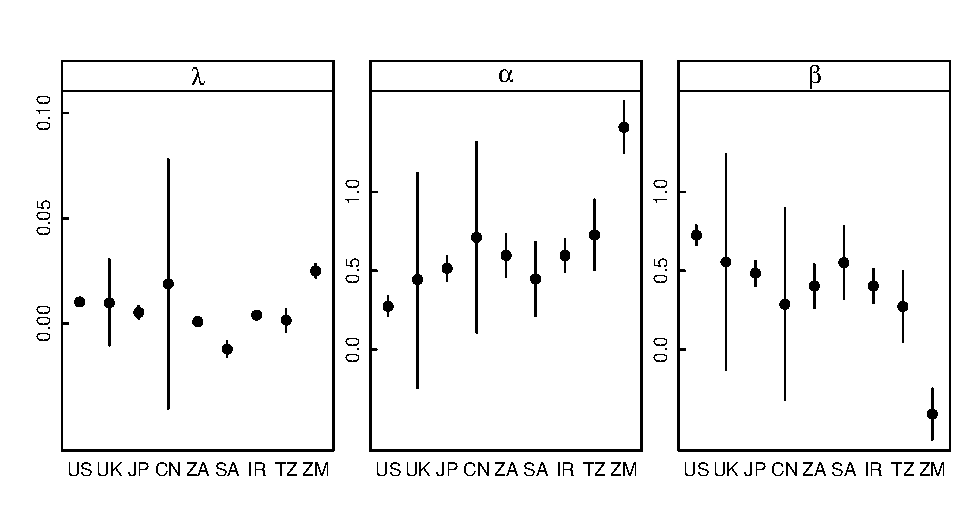
\includegraphics[width=\maxwidth]{figure/CD_Params_Graph} \caption[Cobb-Douglas (without energy) model parameters]{Cobb-Douglas (without energy) model parameters.\label{fig:CD_Params_Graph}}
\end{figure}


\end{knitrout}





\section{Cobb-Douglas With Energy}

We can force $\alpha$, $\beta$, and $\gamma$ to be in $[0,1]$ by a reparameterization:

\[ a \in[0,1], b \in [0,1], \alpha=\min(a,b), \beta=|b-a|, \gamma = 1-\max(a,b) \]




\subsection{Cobb-Douglas with $Q$}







\subsection{Cobb-Douglas With $X$}







\subsection{Cobb-Douglas With $U$}







\section{CES}




\subsection{CES with $Q$}






%% The Appendices part is started with the command \appendix;
%% appendix sections are then done as normal sections
%% \appendix

%% \section{}
%% \label{}

%% References
%%
%% Following citation commands can be used in the body text:
%%
%%  \citet{key}  ==>>  Jones et al. (1990)
%%  \citep{key}  ==>>  (Jones et al., 1990)
%%
%% Multiple citations as normal:
%% \citep{key1,key2}         ==>> (Jones et al., 1990; Smith, 1989)
%%                            or  (Jones et al., 1990, 1991)
%%                            or  (Jones et al., 1990a,b)
%% \cite{key} is the equivalent of \citet{key} in author-year mode
%%
%% Full author lists may be forced with \citet* or \citep*, e.g.
%%   \citep*{key}            ==>> (Jones, Baker, and Williams, 1990)
%%
%% Optional notes as:
%%   \citep[chap. 2]{key}    ==>> (Jones et al., 1990, chap. 2)
%%   \citep[e.g.,][]{key}    ==>> (e.g., Jones et al., 1990)
%%   \citep[see][pg. 34]{key}==>> (see Jones et al., 1990, pg. 34)
%%  (Note: in standard LaTeX, only one note is allowed, after the ref.
%%   Here, one note is like the standard, two make pre- and post-notes.)
%%
%%   \citealt{key}          ==>> Jones et al. 1990
%%   \citealt*{key}         ==>> Jones, Baker, and Williams 1990
%%   \citealp{key}          ==>> Jones et al., 1990
%%   \citealp*{key}         ==>> Jones, Baker, and Williams, 1990
%%
%% Additional citation possibilities
%%   \citeauthor{key}       ==>> Jones et al.
%%   \citeauthor*{key}      ==>> Jones, Baker, and Williams
%%   \citeyear{key}         ==>> 1990
%%   \citeyearpar{key}      ==>> (1990)
%%   \citetext{priv. comm.} ==>> (priv. comm.)
%%   \citenum{key}          ==>> 11 [non-superscripted]
%% Note: full author lists depends on whether the bib style supports them;
%%       if not, the abbreviated list is printed even when full requested.
%%
%% For names like della Robbia at the start of a sentence, use
%%   \Citet{dRob98}         ==>> Della Robbia (1998)
%%   \Citep{dRob98}         ==>> (Della Robbia, 1998)
%%   \Citeauthor{dRob98}    ==>> Della Robbia


%% References with bibTeX database:

\bibliographystyle{model2-names}
\bibliography{<your-bib-database>}

%% Authors are advised to submit their bibtex database files. They are
%% requested to list a bibtex style file in the manuscript if they do
%% not want to use model2-names.bst.

%% References without bibTeX database:

% \begin{thebibliography}{00}

%% \bibitem must have one of the following forms:
%%   \bibitem[Jones et al.(1990)]{key}...
%%   \bibitem[Jones et al.(1990)Jones, Baker, and Williams]{key}...
%%   \bibitem[Jones et al., 1990]{key}...
%%   \bibitem[\protect\citeauthoryear{Jones, Baker, and Williams}{Jones
%%       et al.}{1990}]{key}...
%%   \bibitem[\protect\citeauthoryear{Jones et al.}{1990}]{key}...
%%   \bibitem[\protect\astroncite{Jones et al.}{1990}]{key}...
%%   \bibitem[\protect\citename{Jones et al., }1990]{key}...
%%   \harvarditem[Jones et al.]{Jones, Baker, and Williams}{1990}{key}...
%%

% \bibitem[ ()]{}

% \end{thebibliography}

\end{document}

%%
%% End of file `elsarticle-template-2-harv.tex'.
